


\documentclass[]{beamer}
% Class options include: notes, notesonly, handout, trans,
%                        hidesubsections, shadesubsections,
%                        inrow, blue, red, grey, brown

% Theme for beamer presentation.
\usepackage{beamerthemesplit} 
% Other themes include: beamerthemebars, beamerthemelined, 
%                       beamerthemetree, beamerthemetreebars  

\title{PHY115}    % Enter your title between curly braces
\author{Dynamics of Rotation}                 % Enter your name between curly braces
\institute{Digipen}      % Enter your institute name between curly braces
\date{Spring 2022} 

\begin{document}

% Creates title page of slide show using above information
\begin{frame}
  \titlepage
\end{frame}
%\note{Talk for 30 minutes} % Add notes to yourself that will be displayed when
                           % typeset with the notes or notesonly class options

\section[]{}

% Creates table of contents slide incorporating
% all \section and \subsection commands
\begin{frame}
  \tableofcontents
\end{frame}

%%%%%%%%%%%%%%%%%%%%%%%%%%%%%%%%%%%%%%%%%%%%%%%%%%%%%%%%%%%%%%%%%%%
\section{Torque}




%%%%%%%%%%%%%%%%%%%%%%%%%%%%%%%%%%%%%%%%%%%%%%%%%%%%%%%%%%%%%%%%%%%

\begin{frame}

Torque

\vspace{7mm}

  \begin{columns}[c]
    \column{2in}  % slides are 3in high by 5in wide

    \begin{itemize}
      \item Direction and magnitud of forces $\rightarrow$ affect Translational Motion.
      \item The point of appliclation $\rightarrow$ affects Rotational Motion.
    \end{itemize}
   
    \vspace{7mm}


    \column{2in}
 



    
  \begin{center}
    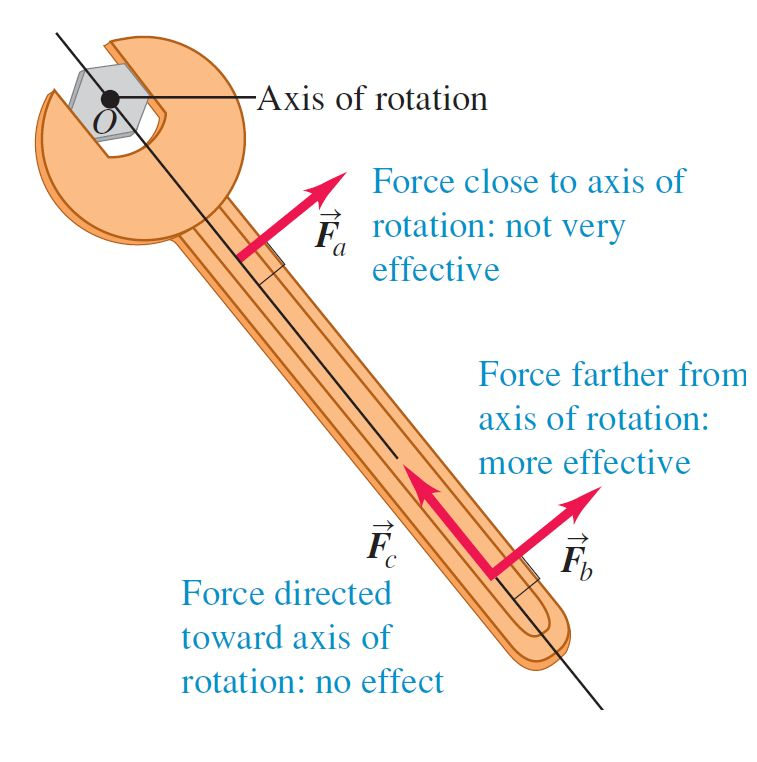
\includegraphics[height=2.in]{images/1.jpg}
  \end{center}

  



    \end{columns}

    \pause

    The quantitative measure of the tendency
    of a force to cause or change a body’s rotational motion is called torque;
    
\end{frame}


%%%%%%%%%%%%%%%%%%%%%%%%%%%%%%%%%%%%%%%%%%%%%%%%%%%%%%%%%%%%%%%%%%%





\begin{frame}



  \begin{columns}[c]
    \column{2in}  % slides are 3in high by 5in wide


    \begin{center}
      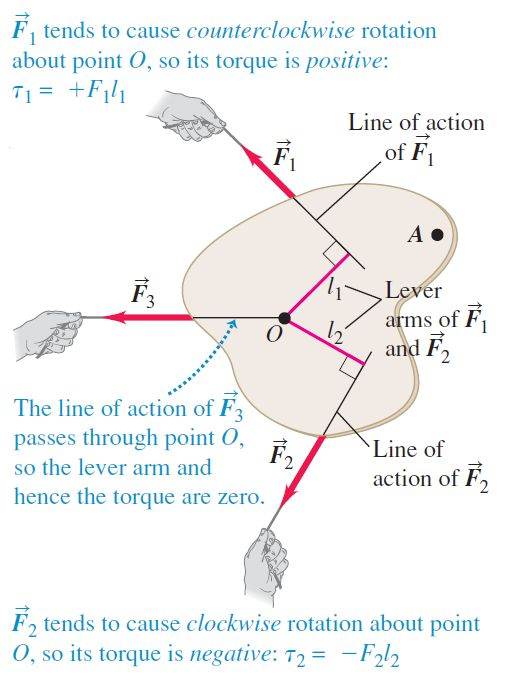
\includegraphics[height=3.0in]{images/2.jpg}
    \end{center}

    


 
    \column{2in}
 



    
    \begin{equation*}
      \tau=F \ell
     \end{equation*}
  
     \begin{equation*}   
      \ell: lever\ arm
  \end{equation*}

\pause

  \begin{equation*}
    \tau_1=+F_1 \ell_1 \ (counterclockwise)
   \end{equation*}

   \pause
  \begin{equation*}
    \tau_2=-F_2 \ell_2 \ (clockwise)
   \end{equation*}


    \end{columns}

    
\end{frame}


%%%%%%%%%%%%%%%%%%%%%%%%%%%%%%%%%%%%%%%%%%%%%%%%%%%%%%%%%%%%%%%%%%%



%%%%%%%%%%%%%%%%%%%%%%%%%%%%%%%%%%%%%%%%%%%%%%%%%%%%%%%%%%%%%%%%%%%





\begin{frame}

EXAMPLE: what is the torque?
\vspace{7mm}


\begin{figure}[h!]  
  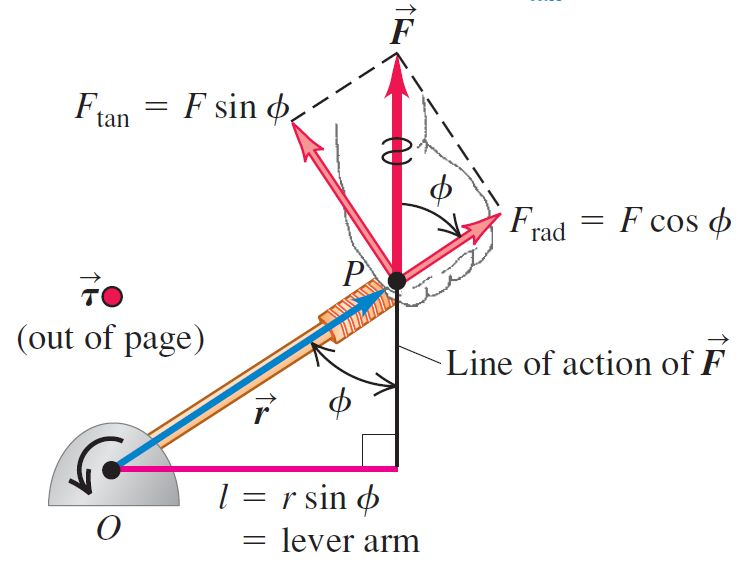
\includegraphics[width=0.6\textwidth]{images/3.jpg}
  \caption{Image from Sears and Zemansky's University Physics With Modern Physics 13th edition. }

\end{figure}

    
\end{frame}


%%%%%%%%%%%%%%%%%%%%%%%%%%%%%%%%%%%%%%%%%%%%%%%%%%%%%%%%%%%%%%%%%%%




\begin{frame}

  EXAMPLE: what is the torque?
  \vspace{7mm}
  

  \begin{equation}
    \boxed{\tau=F\ell=rFsin\Phi}
  \end{equation}
      
  \end{frame}
  
  
  %%%%%%%%%%%%%%%%%%%%%%%%%%%%%%%%%%%%%%%%%%%%%%%%%%%%%%%%%%%%%%%%%%%
  

  \begin{frame}

   TORQUE AS A VECTOR
   
   \vspace{7mm}

\begin{itemize}
  \item Angular velocity $\rightarrow$ vector
   \pause
  \item Angular acceleration $\rightarrow$ vector
  \pause
  \item Torque $\rightarrow$ also a vector
\end{itemize}


  \end{frame}
    
    
    %%%%%%%%%%%%%%%%%%%%%%%%%%%%%%%%%%%%%%%%%%%%%%%%%%%%%%%%%%%%%%%%%%%
    


  %%%%%%%%%%%%%%%%%%%%%%%%%%%%%%%%%%%%%%%%%%%%%%%%%%%%%%%%%%%%%%%%%%%
  \subsection{Torque as a vector}

  \begin{frame}

    TORQUE AS A VECTOR
    
    \vspace{7mm}
 

    \begin{equation}
      \boxed{\vec{\tau}=\vec{r} \times \vec{F}}
    \end{equation}
     
    
    \pause

    \begin{itemize}
      \item Magnitude: $\tau=F\ell=rFsin\Phi$
      \vspace{5mm}
      \item Direction: Right Hand Rule.
      \vspace{5mm}
      \begin{itemize}
        \item $\vec{\tau}$ perpendicular to the plane of $\vec{r}$ and $\vec{F}$
        \item $(\cdot)$ $\rightarrow$ $\vec{\tau}$ points out the screen.
        \item $(\times)$ $\rightarrow$ $\vec{\tau}$ points into the screen.
      \end{itemize}
    \end{itemize}
 
   \end{frame}
     

  %%%%%%%%%%%%%%%%%%%%%%%%%%%%%%%%%%%%%%%%%%%%%%%%%%%%%%%%%%%%%%%%%%%
  
  \begin{frame}


  Test Your Understanding of 
      
  \vspace{7mm}
  
The figure shows a force P being applied to one end of a lever of length $L$. 
\vspace{7mm}


What is the magnitude of the torque of this force about point $A$? 

\begin{enumerate}
  \item $PL sin(\theta)$;
  \item $PL cos (\theta)$;
  \item $PL tan (\theta)$.
\end{enumerate}


\end{frame}



%%%%%%%%%%%%%%%%%%%%%%%%%%%%%%%%%%%%%%%%%%%%%%%%%%%%%%%%%%%%%%%%%%%

\subsection{Torque and Angular Acceleration}


  \begin{frame}

  Torque and Angular Acceleration for a Rigid Body

    
    \vspace{7mm}



    \begin{columns}[c]
      \column{2in}  % slides are 3in high by 5in wide
     
       
    \begin{figure}[h!]  
      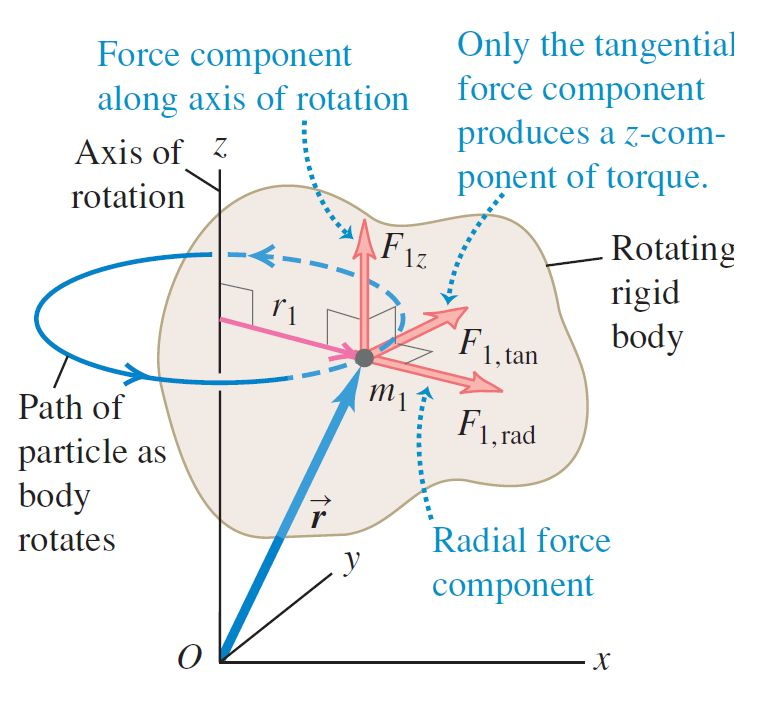
\includegraphics[width=1.3\textwidth]{images/5.jpg}
      \caption{Image from Sears and Zemansky's University Physics With 
      Modern Physics 13th edition. }
    
    \end{figure}

      \column{2in}

\begin{equation*}
  F_{1,tan}=m_1 a_{1,tan}
\end{equation*}

\begin{equation*}
  F_{1,tan}r_1=m_1 r_1 a_{1,tan}=m_1 r^2_1 \alpha_{z}
\end{equation*}

\begin{equation*}
 \rightarrow \sum \tau_{iz}=\left( \sum m_i r^2_i    \right)\alpha_{z}
\end{equation*}
   

      \end{columns}

      


\end{frame}
     


%%%%%%%%%%%%%%%%%%%%%%%%%%%%%%%%%%%%%%%%%%%%%%%%%%%%%%%%%%%%%%%%%%%




\begin{frame}

  Inertia Momentum
  \vspace{7mm}

 \begin{equation}
   I=\left( \sum m_i r^2_i    \right)
 \end{equation}     

 \vspace{7mm}

 \pause

 Then\dots
 \vspace{7mm}

 \begin{equation}
  \sum \tau_{iz}=I \alpha_z
 \end{equation}

 \pause
Just as Newton’s second law says that the net force on a particle equals the particle’s
mass times its acceleration, the net torque on a rigid body equals
the body’s moment of inertia about the rotation axis times its angular acceleration.

\end{frame}


%%%%%%%%%%%%%%%%%%%%%%%%%%%%%%%%%%%%%%%%%%%%%%%%%%%%%%%%%%%%%%%%%%%


\begin{frame}
  Moments of Inertia of Various Bodies
  \vspace{7mm}


\begin{figure}[h!]  
  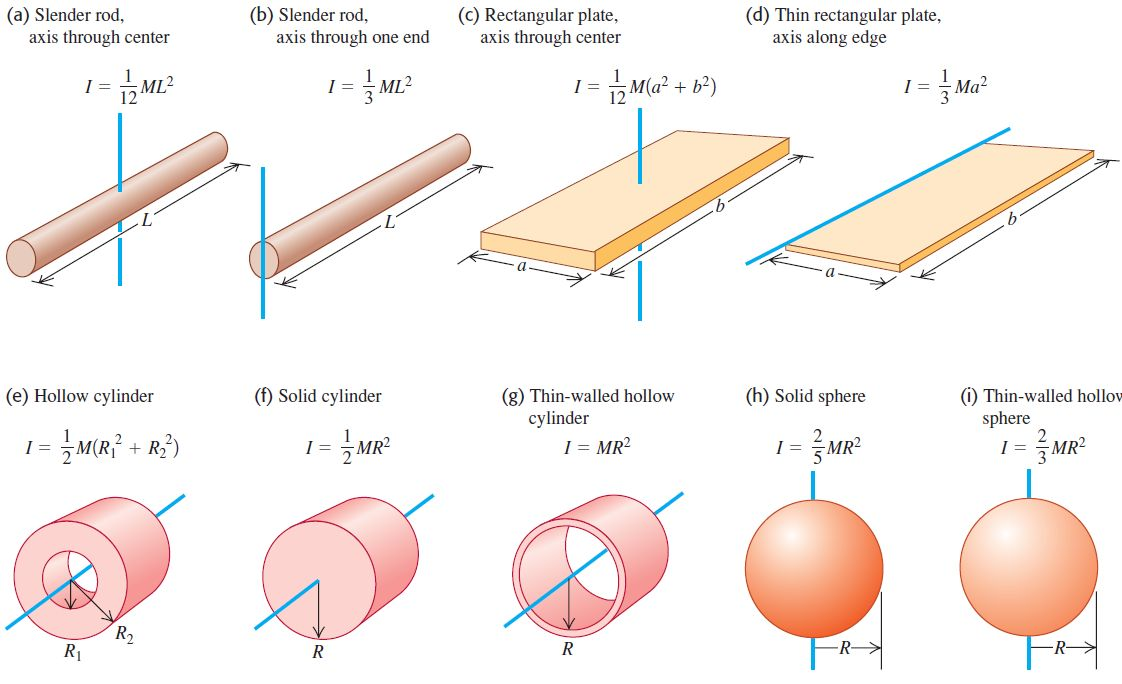
\includegraphics[width=0.9\textwidth]{images/7.jpg}
  \caption{Image from Sears and Zemansky's University Physics With 
  Modern Physics 13th edition. }
\end{figure}


\end{frame}

%%%%%%%%%%%%%%%%%%%%%%%%%%%%%%%%%%%%%%%%%%%%%%%%%%%%%%%%%%%%%%%%%%%




\begin{frame}


  Test Your Understanding of the Section
  \vspace{7mm}

Rank the magnitudes of the following forces that act during the motion, in
  order from largest to smallest magnitude. (i) the tension force (magnitude $T_1$ ) in the horizontal
  part of the string; (ii) the tension force (magnitude $T_2$) in the vertical part of the
  string; (iii) the weight $m_2g$ of the hanging object.


  \begin{figure}[h!]  
    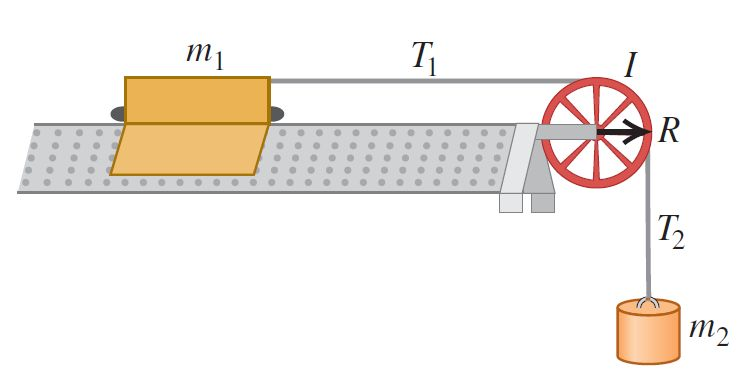
\includegraphics[width=0.7\textwidth]{images/8.jpg}
    \caption{Image from Sears and Zemansky. }
  \end{figure}



\end{frame}



%%%%%%%%%%%%%%%%%%%%%%%%%%%%%%%%%%%%%%%%%%%%%%%%%%%%%%%%%%%%%%%%%%%




\begin{frame}


  Rolling Without Slipping: Motion of a wheel
  \vspace{7mm}

  The motion of a rolling wheel is   the sum of the translational motion of the
  center of mass plus the rotational motion   of the wheel around the center of mass.


  
  \begin{figure}[h!]  
    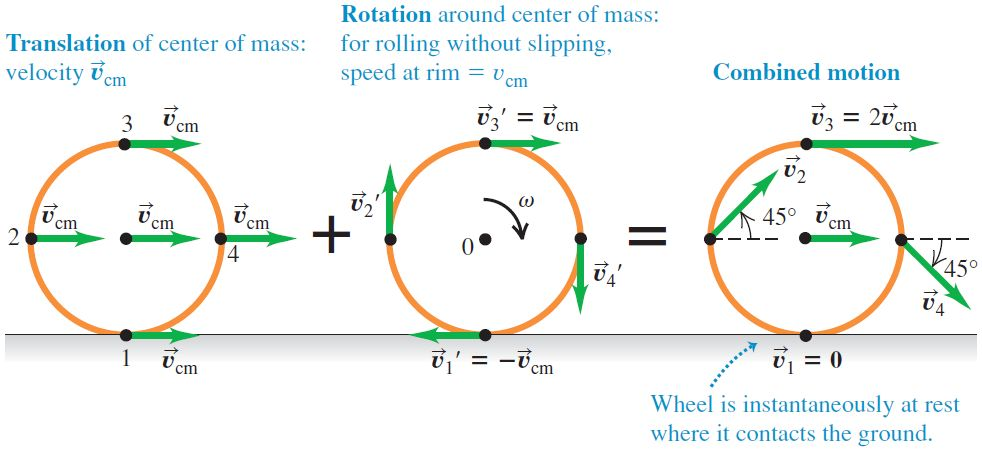
\includegraphics[width=0.9\textwidth]{images/9.jpg}
    \caption{Image from Sears and Zemansky. }
  \end{figure}

\end{frame}



%%%%%%%%%%%%%%%%%%%%%%%%%%%%%%%%%%%%%%%%%%%%%%%%%%%%%%%%%%%%%%%%%%%





\begin{frame}


  Acceleration of a rolling sphere
  \vspace{7mm}

  A bowling ball rolls without slipping down a ramp, which is
  inclined at an angle $\beta$ to the horizontal. What are the
  ball’s acceleration and the magnitude of the friction force on the
  ball? Treat the ball as a uniform solid sphere, ignoring the finger
  holes.


  \begin{figure}[h!]  
    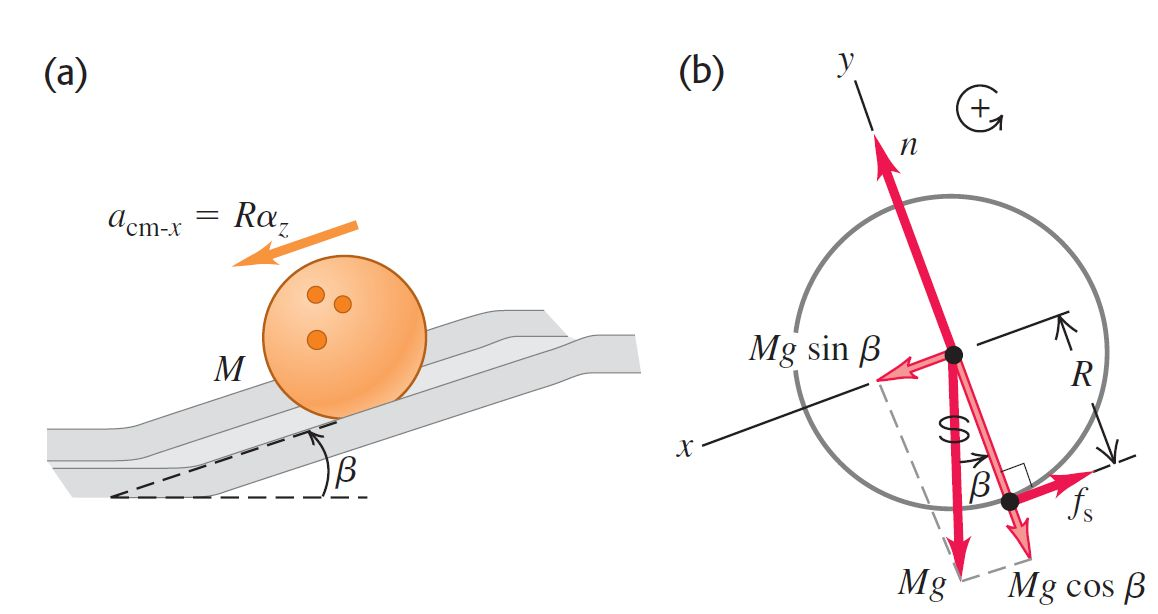
\includegraphics[width=0.7\textwidth]{images/11.jpg}
    \caption{Image from Sears and Zemansky. }
  \end{figure}


\end{frame}

%%%%%%%%%%%%%%%%%%%%%%%%%%%%%%%%%%%%%%%%%%%%%%%%%%%%%%%%%%%%%%%%%%%

\begin{frame}


  Race of the rolling bodies
  \vspace{7mm}

  What shape should a body have to reach the bottom of the
  incline first?


  
  \begin{figure}[h!]  
    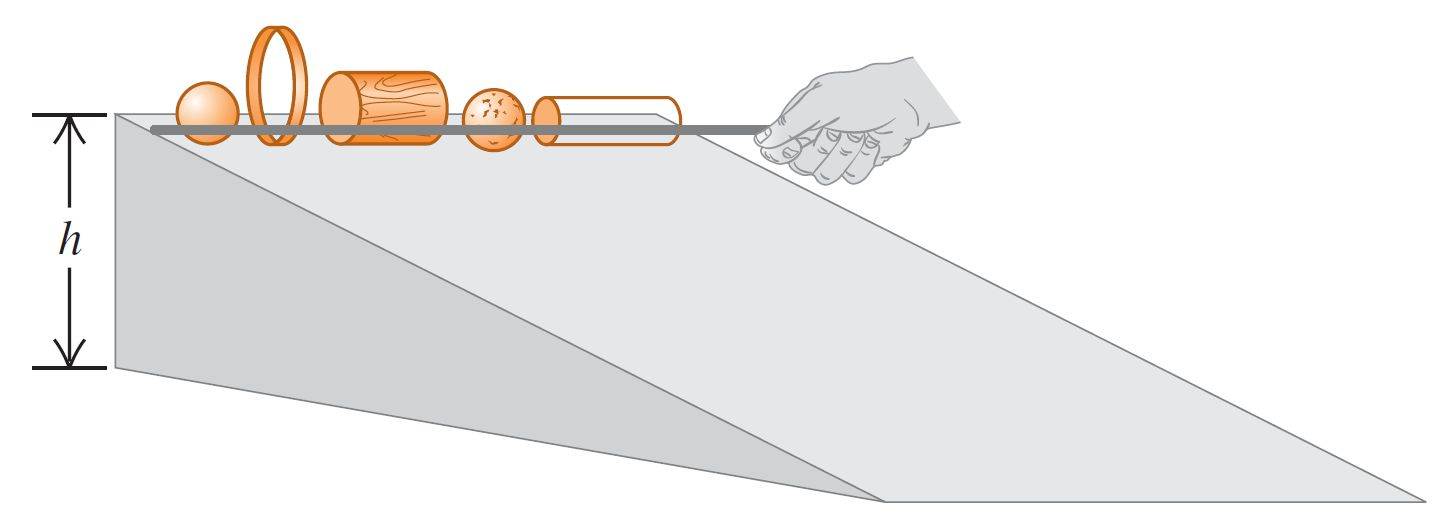
\includegraphics[width=0.9\textwidth]{images/10.jpg}
    \caption{Image from Sears and Zemansky.}
  \end{figure}

\end{frame}



%%%%%%%%%%%%%%%%%%%%%%%%%%%%%%%%%%%%%%%%%%%%%%%%%%%%%%%%%%%%%%%%%%%
\subsection{Angular Momentum}

\begin{frame}


Angular Momentum

\vspace{7mm}

Every rotational quantity that we have encountered last sections is the
analog of some quantity in the translational motion of a particle.

\vspace{7mm}
\pause

$\vec{\tau}\rightarrow\vec{F}$

 \pause

 
 \vspace{7mm}

 The analog of $\vec{P}$ of a particle is angular momentum $\vec{L}$.
 \pause

 \vspace{7mm}


 \begin{equation}
  \vec{L}=\vec{r}\times\vec{p}
 \end{equation}

\end{frame}



%%%%%%%%%%%%%%%%%%%%%%%%%%%%%%%%%%%%%%%%%%%%%%%%%%%%%%%%%%%%%%%%%%%

\begin{frame}


Angular Momentum

\vspace{7mm}



\begin{columns}[c]
  \column{2in}  % slides are 3in high by 5in wide
 

  For a rigid body rotating around a symmetry axis:

  \begin{equation}
    \vec{L}=I\vec{\omega}
   \end{equation}

  \column{2in}


 
  
  
     
   \begin{figure}[h!]  
    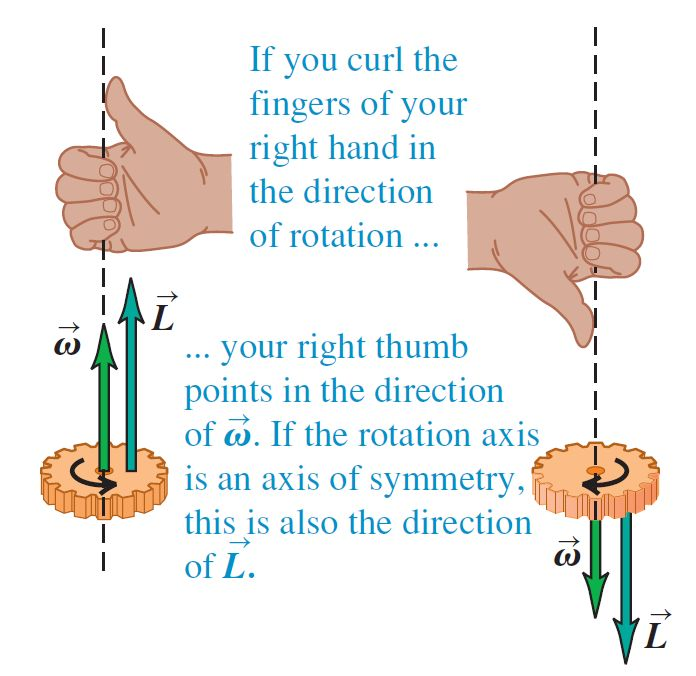
\includegraphics[width=1.2\textwidth]{images/12.jpg}
    \caption{Image from Sears and Zemansky.}
  \end{figure}
  


  \end{columns}




\end{frame}



%%%%%%%%%%%%%%%%%%%%%%%%%%%%%%%%%%%%%%%%%%%%%%%%%%%%%%%%%%%%%%%%%%%

\begin{frame}


  Angular Momentum and Torque
  
  \vspace{7mm}
  
  
  We can show that there is a relation between angular momentum and torque:
  \pause

  \begin{equation}
   \frac{d\vec{L}}{dt} =\sum \vec{\tau}
  \end{equation}
  
  \pause
  When the net external torque acting on a system is zero, the total angular
momentum of the system is constant (conserved).
  
\pause
\vspace{7mm}
No external torque $\rightarrow$ $\vec{L}=constant$ $\rightarrow$ $\omega I=constant$
  
  \end{frame}


%%%%%%%%%%%%%%%%%%%%%%%%%%%%%%%%%%%%%%%%%%%%%%%%%%%%%%%%%%%%%%%%%%%

\begin{frame}

  Test Your Understanding of Section

  \vspace{7mm}


  If the polar ice caps were to completely
melt due to global warming, the melted ice would redistribute itself over the earth.
This change would cause the length of the day (the time needed for the earth to rotate
once on its axis) to
\vspace{7mm}

\begin{enumerate}
  \item increase;
  \item decrease;
  \item remain the same.
\end{enumerate}
\vspace{7mm}

 (Hint: Use angular
momentum ideas. Assume that the sun, moon, and planets exert negligibly small torques
on the earth.)

  
  \end{frame}


%%%%%%%%%%%%%%%%%%%%%%%%%%%%%%%%%%%%%%%%%%%%%%%%%%%%%%%%%%%%%%%%%%%

\begin{frame}

  Test Your Understanding of Section

  \vspace{7mm}


  A ball is attached to one end of a
piece of string. You hold the other end of the string and whirl the ball in a circle around
your hand. 
\vspace{7mm}

\begin{enumerate}
  \item If the ball moves at a constant speed, is its linear momentum constant?
Why or why not?
\item  Is its angular momentum constant? Why or why not? 
\end{enumerate}


  
  \end{frame}



%%%%%%%%%%%%%%%%%%%%%%%%%%%%%%%%%%%%%%%%%%%%%%%%%%%%%%%%%%%%%%%%%%%

\begin{frame}

  Gyroscopes 

  \vspace{7mm}


   \begin{figure}[h!]  
    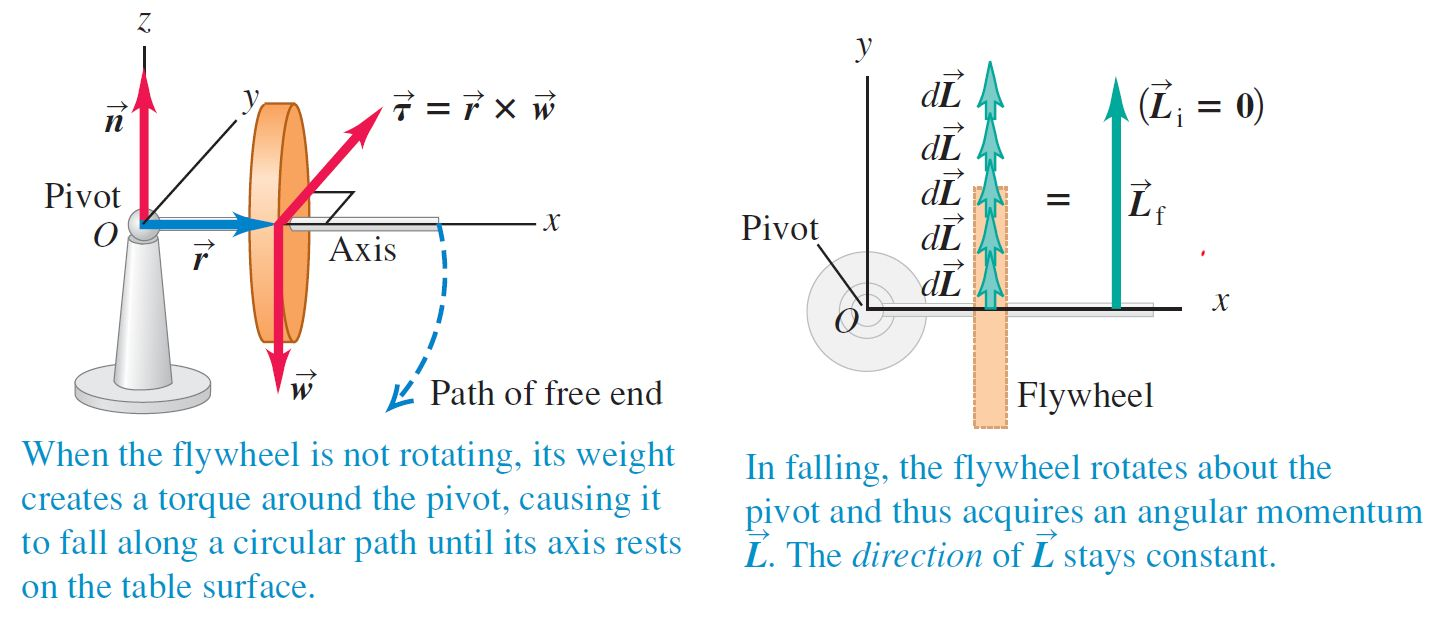
\includegraphics[width=1.2\textwidth]{images/13.jpg}
    \caption{Image from Sears and Zemansky.}
  \end{figure}
  
  \end{frame}

%%%%%%%%%%%%%%%%%%%%%%%%%%%%%%%%%%%%%%%%%%%%%%%%%%%%%%%%%%%%%%%%%%%

\begin{frame}

  Gyroscopes 

  \vspace{7mm}


   \begin{figure}[h!]  
    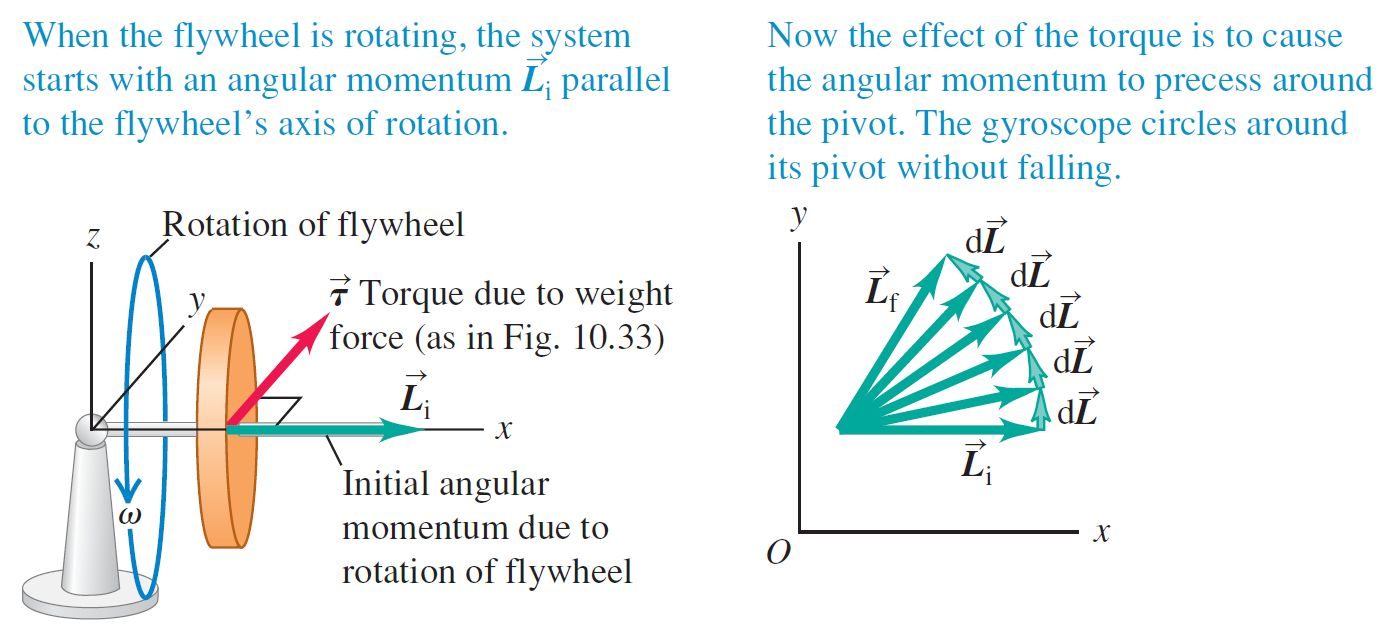
\includegraphics[width=1.2\textwidth]{images/14.jpg}
    \caption{Image from Sears and Zemansky.}
  \end{figure}
  
  \end{frame}





%%%%%%%%%%%%%%%%%%%%%%%%%%%%%%%%%%%%%%%%%%%%%%%%%%%%%%%%%%%%%%%%%%%

\begin{frame}

\begin{enumerate}
\item Can a single force applied to a body change both its translational
and rotational motion? Explain.
\pause
\item When an acrobat walks on a tightrope, she extends her arms
straight out from her sides. She does this to make it easier for her
to catch herself if she should tip to one side or the other. Explain
how this works.
\pause

\item Experienced cooks can tell whether an egg is raw or hardboiled
by rolling it down a slope (taking care to catch it at the bottom).
How is this possible? What are they looking for?



\end{enumerate}
  
  \end{frame}


%%%%%%%%%%%%%%%%%%%%%%%%%%%%%%%%%%%%%%%%%%%%%%%%%%%%%%%%%%%%%%%%%%%


%%%%%%%%%%%%%%%%%%%%%%%%%%%%%%%%%%%%%%%%%%%%%%%%%%%%%%%%%%%%%%%%%%%

\begin{frame}

Example 1
  \vspace{7mm}

  \begin{columns}[c]
    \column{2in}  % slides are 3in high by 5in wide
   

A square metal plate $0.180 m$ on each side is pivoted
about an axis through point $O$ at its center and perpendicular to the
plate. Calculate the net torque about this axis due to
the three forces shown in the figure if the magnitudes of the forces
are $F_1=18N$, $F_2=26N$  and $F_3=14N$  The plate and
all forces are in the plane of the page. The plate and
all forces are in the plane of the screen.


    \column{2in}
 

    \begin{figure}[h!]  
      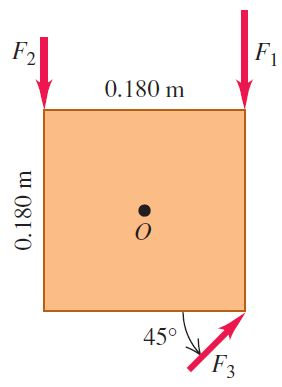
\includegraphics[width=0.8\textwidth]{images/16.jpg}
      \caption{Image from Sears and Zemansky.}
    \end{figure}

    

    \end{columns}





  \end{frame}


%%%%%%%%%%%%%%%%%%%%%%%%%%%%%%%%%%%%%%%%%%%%%%%%%%%%%%%%%%%%%%%%%%%







%%%%%%%%%%%%%%%%%%%%%%%%%%%%%%%%%%%%%%%%%%%%%%%%%%%%%%%%%%%%%%%%%%%

\begin{frame}

Example 2
  \vspace{7mm}


  \begin{columns}[c]
    \column{2.2in}  % slides are 3in high by 5in wide
   

    A small block on a
 horizontal surface ($\mu=0$)
withmass  $0.025kg$ is
attached to a massless cord passing
through a hole. The block is originally
revolving at a distance of
$0.3m$ from the hole with $\omega = 1.75~rad/s$. The
cord is then pulled from below,
shortening the radius 
to $0.15 m$. (a) Is the angular momentum
of the block conserved? (b) What is the new
angular speed? 


    \column{2in}
 


    \begin{figure}[h!]  
      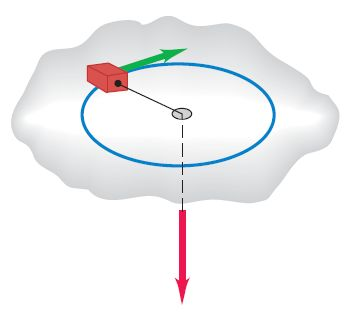
\includegraphics[width=1.1\textwidth]{images/17.jpg}
      \caption{Image from Sears and Zemansky.}
    \end{figure}



    \end{columns}





  \end{frame}



%%%%%%%%%%%%%%%%%%%%%%%%%%%%%%%%%%%%%%%%%%%%%%%%%%%%%%%%%%%%%%%%%%%

\begin{frame}

Example 3
  \vspace{7mm}



  A cue ball ( mass $m$, radius $R$) is at
  rest on a level pool table. You give the ball a
 horizontal hit of magnitude $F$ at a height $h$ above the center
  of the ball. The force of the hit is much greater
  than the friction force $ƒ$.
  The hit lasts for a short time $\Delta t$ . (a) For what value of
  $h$ will the ball roll without slipping? (b) If you hit the ball 
  center ($h=0$), the ball will slide across the table for a while, but
  eventually it will roll without slipping. What will the speed of its
  center of mass be then?
  
  \begin{figure}[h!]  
    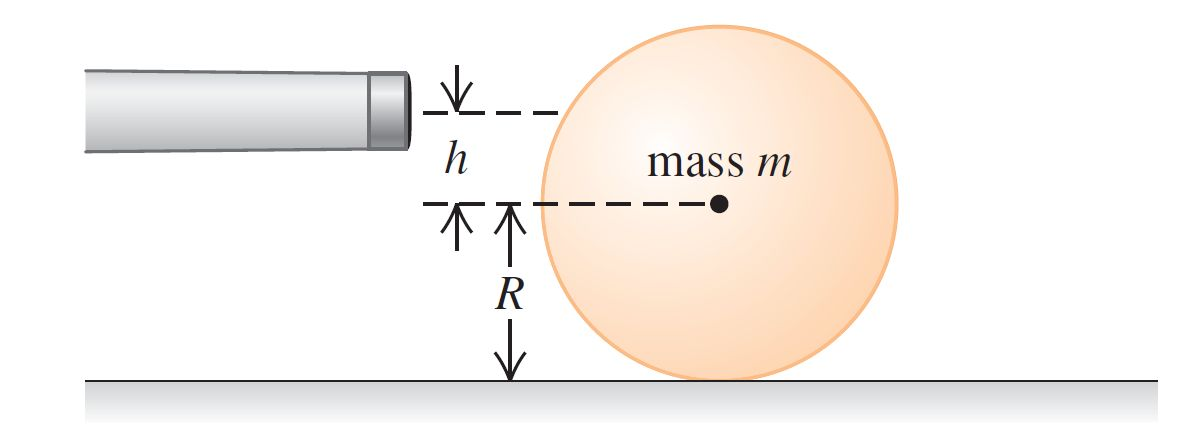
\includegraphics[width=0.8\textwidth]{images/15.jpg}
    \caption{Image from Sears and Zemansky.}
  \end{figure}


  \end{frame}


%%%%%%%%%%%%%%%%%%%%%%%%%%%%%%%%%%%%%%%%%%%%%%%%%%%%%%%%%%%%%%%%%%%









%%%%%%%%%%%%%%%%%%%%%%%%%%%%%%%%%%%%%%%%%%%%%%%%%%%%%%%%%%%%%%%%%%%
 \end{document}
%%%%%%%%%%%%%%%%%%%%%%%%%%%%%%%%%%%%%%%%%%%%%%%%%%%%%%%%%%%%%%%%%%%